\documentclass[a4paper,abstract=on]{scrartcl}

%
% Packages
%
\usepackage[paper=a4paper,top=2cm,left=2cm,right=1.5cm,bottom=2cm,foot=1cm]{geometry} % Margins
\usepackage[utf8]{inputenc} % encoding
\usepackage[T1]{fontenc}    % language
\usepackage[english]{babel} % language
\usepackage{todonotes}      % to keep track of stuff
\usepackage{graphicx}       % images
\usepackage{epstopdf}       % support for EPS images
\usepackage{indentfirst}    % indent first paragraph
\usepackage{relsize}        % relative font sizes
\usepackage[colorlinks=true,linkcolor=black,citecolor=black]{hyperref} % pretty urls
\usepackage[noabbrev,capitalise]{cleveref}       % better references
\usepackage{datetime}       % date & time helpers
\usepackage{xspace}         % spacing helper for macros
\usepackage{suffix}         % for making multi-versioned commands

% pseudo-code environments
\usepackage{algpseudocode}
\usepackage{algorithmicx}
\usepackage{algorithm}

% IEEE tools
\usepackage[retainorgcmds]{IEEEtrantools}




%
% Configs
%

% use the images/ dir
\graphicspath{{../img/}}

%
% Custom commands
%

% todo[inline]
\newcommand\todox[1]{\todo[inline]{#1}}

% text aliases
\newcommand{\GAMA}{\texttt{GAMA}\xspace}          % GAME
\newcommand{\hetplat}{\textit{HetPlat}\xspace}    % HetPlat
\newcommand{\hetplats}{\textit{HetPlats}\xpspace} % HetPlats

% roles
\newcommand{\role}[1]{\smaller{\textit{(#1)}}}
\newcommand{\student}{\role{Student}}
\newcommand{\advisor}{\role{Advisor}}
\newcommand{\coadvisor}{\role{Co-Advisor}}

% Force paragraph indentation
\newlength{\paragraphindentationlength}
\setlength{\paragraphindentationlength}{\parindent}
\newcommand\sudoindent{\hspace{\paragraphindentationlength}}

% email
\newcommand{\linklike}[1]{{\smaller\smaller\ttfamily #1}}
\newcommand\email[1]{\href{mailto:#1}{\linklike{#1}}}
\WithSuffix\newcommand\email*[2]{\href{mailto:#1}{\linklike{#1}}}

% signature space
\newcommand{\sigspace}[2]{

\begin{minipage}{\textwidth}%
\vspace{2cm}%
\begin{tabular*}{.6\textwidth}{@{\extracolsep{\fill}}lr}
\hline
{#1} & #2
\end{tabular*}%
\end{minipage}%
}


\titlehead{%
University~of~Minho\hfill Informatics~Department%
}

\subject{Dissertation for Master’s Degree in Informatics Engineering}

\author{%
Miguel~Palhas\\\student\\\email{pg19808@alunos.uminho.pt}%
\and Alberto~Proença\\\advisor\\\email{aproenca@di.uminho.pt}%
\and Luis~Paulo~Santos\\\coadvisor\\\email{psantos@di.uminho.pt}%
}

\title{XXXXXXXXXXXXXXXXXX}

\date{Braga, November 2012}


\begin{document}

  %
  % Title
  %
  \maketitle

  %
  % Content
  %
  \begin{abstract}

High performance computing has suffered several recent changes, with the evolution of Heterogeneous Platforms, where multiple devices with different architectures are able to share workload of increase performance.
Several frameworks have been in development, to aid the programmer in using these platforms, by dynamically distributing workload. One of these is the GAMA framework, designed to deal with irregular applications, by unifying the multiple execution and memory models of each device into a single, hardware independent model. GAMA handles the workload distribution across multiple computational resources, and attempts to balance them based on measurements from previous executions, with the main goal of maximizing efficiency. So far, this framework has only been tested for small benchmark kernels, for comparison with similar alternatives using standardized algorithms, but still lacks a deeper study, using a more realistic case study, to better understand its limitations.

The subject of this dissertation is to provide a more in-depth evaluation of GAMA, using the progressive photon mapping algorithm as a case study. The goal is to validate its effectiveness with a full sized application, and identify points of improvement, not only with the analysis of the case study, but also via comparison with similar frameworks. 
\end{abstract}

  \section{Context}

Current high performance computing platforms are composed of different architectures working together to deliver a higher computational power. These platforms, usually called Heterogeneous Platforms, typically consist of one or more multi-core CPU, and other types of devices, such as massively parallel architectures like Graphical Processing Units (GPUs), or event more specialized architectures like Field-Programmable Gate Arrays (FPGAs) or Digital Signal Processors (DSPs).

Using different devices to share the workload and achieve a higher performance can be a challenging task, since each platform has very specific characteristics, and usually requires specific programming and memory models to effectively take advantage of the specialized hardware. Algorithms often have to be adapted as well, or even replaced, to run efficiently on a specific platform. Input data may also play a role, as the same algorithm applied to different inputs may also have completely different behaviours.

When dealing with a HetPlat, an additional concern arises, related to the memory space. In a HetPlat, each device usually has its own local memory space, and requires communication operations to transfer between the local memory and the global system memory. This means that the programmer must be careful not only to adapt the programming model to each device, but it also to be concerned about the cost to move data back and forth, which can introduce an additional bottleneck in the execution, and even hide completely.

Due to these issues, enabling an application to correctly take advantage of all the available resources of a HetPlat can become a challenging problem. A balance must be achieved between the tasks and the resources, assigning each available task to the platform that will most likely achieve better performance at any given moment.

To tackle this problem, several frameworks have been proposed which  attempt to hide some of this difficulties. Some of these include StarPU \cite{augonnet2011starpu}, Harmony \cite{diamos2008harmony} and GAMA \cite{joao2012gama}. These frameworks attempt to address problems such as memory management, or the scheduling of the multiple tasks issued for execution.

Most of these frameworks however, provide mechanisms suited mostly for regular applications. When dealing with irregular applications, problems like scheduling become even more difficult, in particular because memory usage patterns are less predictable. This directly affects the decisions of the scheduler, and as such must be taken into account by the performance model employed by the framework, as explained in \cite{artur2012gama}. Irregular applications are one of the targets of the GAMA framework, which will be the main focus of this dissertation, and is explained more deeply in \Cref{sec:gama}.


\subsection{GAMA}

The GAMA (GPU And Multicore Aware) framework is a tool that provides the mechanisms required to efficiently execute data-parallel applications in a Heterogeneous Platform. It works as an abstraction layer above the hardware, moving the programmer away from the task of scheduling the workload across the multiple resources available. In GAMA, an application is a collection of ordered jobs, each of which is composed of several tasks that are applied to different data sets. All memory is abstracted into a global address space, working as a distributed shared memory system \cite{ricardo2012gama}


  \section{GAMA}
\label{sec:gama}

The GPU And Multi-core Aware (GAMA) framework is a tool that provides the mechanisms required to efficiently execute data-parallel applications in a Heterogeneous Platform. It works as an abstraction layer above the hardware, employing an execution and memory model that allows the developer to remain agnostic of the available devices and other resources, focusing more on the algorithm itself, while also allowing lower level tuning of the algorithms for each specific device, if required.

The main goal of GAMA is not to provide a replacement to the current set of different programming models that are found on a HetPlat, but to create a layer above them to automatically deal with the more generic aspects such as task scheduling, memory management and coordination.

\subsection{Execution Model}

GAMA employs a task-based Unified Programming and Execution Model (UPEM) to create an abstraction of the different models of the underlying devices on a HetPlat. This model organizes available hardware using three concepts:

\begin{description}
  \item[Computational Unit] (CU) Name given to an individual processing element, capable of performing generic computations;

  \item[Device] The group of all Computational Units with a common programming model and a common private memory address space;

  \item[Host] The group of all Devices within a single computing node.
\end{description}

This organization of the execution model ensures that each device contains only CU's with the same memory address space, allowing for the usage of device-specific synchronization mechanisms to manage the coordination of concurrent executions within that device.

A basic implementation of an algorithm with GAMA requires at least two methods: a kernel and a dice. These two method together form what is known by GAMA as a job. The kernel is analogous to a CUDA kernel, as it defines the code that will be executed in each thread. A dice method is a way to split the input domain across multiple tasks. It is somewhat analogous the ability of defining task granularity when using OpenMP, but it can employ more flexible solutions, to account for the irregularity of the algorithms.

\subsection{Memory Model}

While at the device level, synchronization is allowed via device-specific mechanics, that is not the case at the host level. When considering the whole host, or the entire group of available devices, a problem arises as each device possesses its own private memory address space, creating an obstacle to efficiently take advantage of the computational resources. Thus, a Global Memory System (GMS) is employed, using a relaxed consistency model requiring explicit memory fences to ensure full data consistency. 

\begin{figure}[!htp]
  \centering
  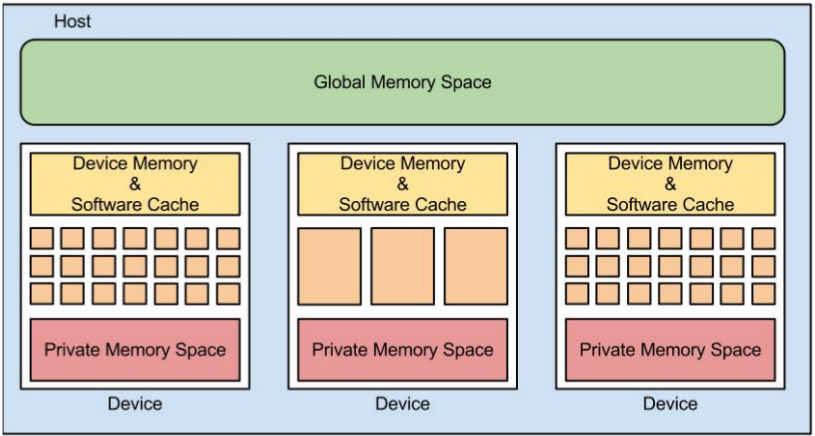
\includegraphics[width=0.6\columnwidth]{UPEM.png}
  \caption{GAMA Memory and Execution Model}
  \label{fig:upem}
\end{figure}

\Cref{fig:upem} provides an overview of the memory model employed in GAMA. It is based on a hierarchy, composed of three levels:
\begin{itemize}
  \item The first level is private and refers to a memory space addressable only by a single task
  \item The second level is shared between all Computational Units of a single device, and thus can be shared across tasks that are running on the same device. It is not addressable by other devices, however.
  \item Finally, the global level is addressable by the entire host system. However, due to implementation details of atomic operations being undefined, this level uses a relaxed consistency model, and requires explicit synchronization barriers to be used in order to ensure data consistency. 
\end{itemize}

Besides the memory hierarchy, GAMA also employs a software cache to reduce latency in global memory space accesses and to exploit potential temporal and spatial locality. This cache is typically implemented over the private memory address space of each device, and can also operate as a pre-fetch mechanism, as it has the ability of copying memory blocks to the device in which they are required, prior to the execution of the corresponding task.


  \section{Progressive Photon Mapping}
\label{sec:photon}

The realistic simulation of illumination of an environment is a complex problem. In theory, a simulation is truly realistic when it completely simulates, or closely approximates, the rendering equation \cite{kajiya1986rendering}. This equation is based on the laws of conservation of energy, and describes the total amount of emitted light from any given point, based on incoming light and reflection distribution, and is described as follows:

\begin{figure}[!htp]
  \begin{equation}
    L_s(x, \Psi_r) = L_e(x, \Psi_r) + \int\limits_\Omega f_r(x, \Psi_i; \Psi_r) L_i(x, \Psi_i) cos\Theta_i \mathrm{d}\omega_i
  \end{equation}
  \label{eq:render}
\end{figure}

In short, the equation defines the surface radiance $L_s(x, \Psi_r)$, leaving the point $x$ in the direction $\Psi_r$ 
This is given by $L_e$, which represents light emitted by a surface, and $L_i$, which is the radiance along the direction given by $\Psi_i$. $f_r$ is the Bidirectional Reflectance Distribution Function (or BRDF) and $\Theta$ is the domain of incoming directions, which is given by a sphere centered on the point $x$. 

Prior to Photon Mapping, typical approaches would include more than one method to approximate the rendering equation, such as Ray Tracing or Radiosity. Each method attempts to simulate the travel of light particles across the scene, and model the various interactions with the environment, but with different approaches and limitations.

Ray Tracing methods work by simulating light particles traveling from the eye into the scene, being reflected and refracted until they reach a light source. 

Radiosity follows an opposite approach, and simulates the path light takes from the light source, until it reaches the eye. It only deals with diffuse interactions, however, and is commonly used in combination with other techniques.

Photon Mapping is another method of approximating the rendering equation \cite{jensen1996global}, and works in a two pass way.
In a first pass, a photon map is constructed by emitting photons from the light sources in the scene. This follows a method similar to Ray Tracing, but every interaction of a photon with the scene is stored in the photon map, creating a structure that roughly represents the entirety of light within the scene.
In the second pass, the final image is rendered by using common Ray Tracing techniques (for example, Monte Carlo ray tracing). The photon map is then used to aid in the computation of the total radiance.
The usage of the photon map is useful not only to increase performance, mostly by allowing a reduction in the number of samples to cast without affecting the final render, but also to allow the modeling of some light effects that are not present, or are inefficient, in other rendering methods, such as caustics or subsurface scattering.

Lastly, Progressive Photon Mapping is an extension to the previous method, that allows arbitrary accuracy not limited by memory \cite{hachisuka2008progressive}. In this method, a multi-pass algorithm is employed, where the first pass consists of a ray tracing method, and all subsequent passes use photon tracing to compute a photon map which will contribute to the global illumination.

The main advantage of this approach is that there is no actual need to store the entire photon map as it is created. Unlike standard photon mapping, it is possible to progressively arbitrarily increase the accuracy of the global illumination without being limited by the amount of memory.

Rendering methods such as photon mapping are a common example of resource demanding, irregular applications, due to the amount of information required to accurately describe a three-dimensional scene, and to realistically simulate all of its lighting effects. Therefore, it should serve a suitable case study for the GAMA framework

  \section{Objectives}

The main goal of this dissertation is to perform a quantitative and qualitative analysis of the GAMA framework, applied to a large scale irregular algorithm, in order to validate its effectiveness, and identify possible soft-spots, especially when compared to other similar frameworks. The work will be focused on fully understanding GAMA, how to better take advantage of it, and possibly how to improve it even further. 

This will be accomplished by using GAMA to implement a computational intensive, irregular application. The results will be used to evaluate the overall efficiency of the GAMA framework, applied to a large scale application, instead of only a single computational kernel. The selected test case for this dissertation was the Progressive Photon Mapping Algorithm, which was described in \Cref{sec:photon}

A comparative analysis will be made between the developed implementation of the algorithm against existing implementations, to assert whether the GAMA framework does a good job at handling a resource intensive application like the progressive photon mapping algorithm.

The work will also be useful to understand how to better take advantage of GAMA, and where it should be improved. An analysis of the execution results of the application should provide insight about the way GAMA is handling the existing jobs and data structures, and from there, identify possible bottlenecks or situations where an improvement could be possible.
The comparative analysis will also be of extreme usefulness in this process, as it will make it possible to know whether or not different implementations perform better than the GAMA implementation, and why. 

  \section{Methodology}

In a first stage, the main focus will be in the research and study of the progressive photon mapping algorithm to better comprehend its details, and in experimental work with GAMA to fully understand the framework. Some time will also be spent studying existing implementations of the case study.

The second stage will focus on implementing the test case using GAMA. This is expected to be the most time consuming task, and a good understanding of the algorithm from the previous stage will be essential.  Other implementations will also be studied, not only to assist in the development, but also to serve as a comparison basis for future analysis.

  In the third stage, a deeper analysis will be done, which should be assisted by the previously gained knowledge. This stage will be essential to determine the effectiveness of GAMA, and to understand how to develop it further.

It will also be interesting, if time allows it, to study the possibilities and limitations of extending GAMA by providing support for additional architectures other than GPU's.

  \section{Timings}

\begin{itemize}
  \item \textbf{November 2012 to December 2012:}

    \sudoindent Literature search on Progressive Photon Mapping;

    \sudoindent Initial studies and hands-on of the GAMA framework.


  \item \textbf{January 2013 to March 2013:}

    \sudoindent Implementation of the Progressive Photon Mapping algorithm.


  \item \textbf{April 2013 to May 2013:}

    \sudoindent Comparative evaluation with other implementations;

    \sudoindent Quantitative and Qualitative analysis of GAMA.


  \item \textbf{June 2013}

      \sudoindent Dissertation writing.
\end{itemize}



  %
  % Bibliography
  %
  \bibliographystyle{../common/IEEE}
  \nocite*{}
  \bibliography{bib/gama,bib/photon_mapping}

  \appendix
  \section{Signatures}

\sigspace{\student}{Miguel~Branco~Palhas}
\sigspace{\advisor}{Alberto~Proença}
\sigspace{\coadvisor}{Luis~Paulo~Santos}


\end{document}
